\section*{TP 12: Physique statistique de particules identiques}
\begin{itemize}
	\item Si le nombre de \(p^++e^-+n\) est (\textbf{im})pair \(\rightarrow\) (\textbf{fermion})boson.
	\item Distribution des fermions (spin demi-entier, toujours \(<1\) par principe d'exclusion de Pauli)
	\begin{equation}
	f^{FD}(E)=\frac{1}{\exp\left[\left(E-\mu\right)/(k_b T)\right]+1}
	\end{equation}
	où \(\mu\) est le potentiel chimique.
\begin{figure}[H]
	\centering
	\begin{tikzpicture}
	\begin{axis}[
	domain=0:10,
	samples=300,
	xmax=10.5,
	ymax=1.1,
	axis lines=left,
	xlabel=\(E\),
	ylabel=\(f^{FD}\),
	ytick={0,0.5,1},
	xtick={0,5},
	xticklabels={0,\(\mu\)},
	legend entries={\(T_1\),\(T_2\),\(T_3\)},
	cycle list name=color list,
	every axis x label/.style={
		at={(ticklabel* cs:1.05)},
		anchor=west,
	},
	every axis y label/.style={
		at={(ticklabel* cs:1.05)},
		anchor=south,
	},
	]
	\addplot{1/(exp((x-5)/0.001)+1)};
	\addplot{1/(exp((x-5)/0.1)+1)};
	\addplot{1/(exp((x-5)/1)+1)};
	\end{axis}
	\end{tikzpicture}
	\caption{Distribution de fermions (\(0<T_1<T_2<T_3\))}
\end{figure}
	\item Distribution de bosons (spin entier, \(\mu<0\))
	\begin{equation}
	f^{BE}(E)=\frac{1}{\exp\left[(E-\mu)/(k_bT)\right]-1}
	\end{equation}
\begin{figure}[H]
	\centering
	\begin{tikzpicture}
	\begin{axis}[
	ymax=2,
	axis lines=left,
	xlabel=\(E\),
	ylabel=\(f^{FD}\),
	domain=0:10,
	samples=300,
	ticks=none,
	legend entries={\(\mu_1\),\(\mu_2\),\(\mu_3\)},
	cycle list name=color list,
	every axis x label/.style={
		at={(ticklabel* cs:1.05)},
		anchor=west,
	},
	every axis y label/.style={
		at={(ticklabel* cs:1.05)},
		anchor=south,
	},
	]
	\addplot{1/(exp((x+0.1))-1)};
	\addplot{1/(exp((x+1))-1)};
	\addplot{1/(exp((x+2))-1)};
	\end{axis}
	\end{tikzpicture}
	\caption{Distribution de bosons (\(\mu_3<\mu_2<\mu_1<0\))}
\end{figure}

	\item Loi de Planck (corps noir)
	\begin{equation}
	u(\nu,T)=\frac{8\pi h \nu^3}{c^3}\frac{1}{\exp\left[h\nu/(k_bT)\right]-1}
	\end{equation}
	\item Énergie libre de Helmholtz: \(F=-k_b T\ln(Z)\) et \(S=-\left(\frac{\partial F}{\partial T}\right)_{V,N}\)
\begin{figure}[H]
	\begin{tikzpicture}
	\draw (3,2) node {Émission spontanée};
	\draw (0,1) node[above]{\(E_j\)}--(2,1) node[midway]{\textbullet};
	\draw (0,0) node[below]{\(E_i\)}--(2,0);
	\draw (4,1) node[above]{\(E_j\)}--(6,1);
	\draw (4,0) node[below]{\(E_i\)}--(6,0) node[midway]{\textbullet};
	\draw[dashed,->] (5,1)--(5,0.15);
	\draw (5,0.5) node[right]{\(\to\gamma\)};
	\draw (9,0.5) node{\(\dfrac{dN_i}{dt}=-\dfrac{dN_j}{dt}=A_{ji}N_j\)};
	\end{tikzpicture}
\end{figure}
\begin{figure}[H]
	\begin{tikzpicture}
	\draw (3,2) node {Absorption};
	\draw (0,1) node[above]{\(E_j\)}--(2,1);
	\draw (0,0) node[below]{\(E_i\)}--(2,0) node[midway]{\textbullet};
	\draw (4,1) node[above]{\(E_j\)}--(6,1) node[midway]{\textbullet};
	\draw (4,0) node[below]{\(E_i\)}--(6,0);
	\draw[dashed,<-] (5,0.85)--(5,0);
	\draw (1,0.5) node[left]{\(\to\gamma\)};
	\draw (9,0.5) node{\(\dfrac{dN_i}{dt}=-\dfrac{dN_j}{dt}=-B_{ji}u(\nu,T)N_j\)};
	\end{tikzpicture}
\end{figure}
\begin{figure}[H]
	\begin{tikzpicture}
	\draw (3,2) node {Émission induite};
	\draw (0,1) node[above]{\(E_j\)}--(2,1) node[midway]{\textbullet};
	\draw (0,0) node[below]{\(E_i\)}--(2,0);
	\draw (4,1) node[above]{\(E_j\)}--(6,1);
	\draw (4,0) node[below]{\(E_i\)}--(6,0) node[midway]{\textbullet};
	\draw[dashed,->] (5,1)--(5,0.15);
	\draw (1,0.5) node[left]{\(\to\gamma\)};
	\draw (5,0.75) node[right]{\(\to\gamma\)};
	\draw (5,0.25) node[right]{\(\to\gamma\)};
	\draw (9,0.5) node{\(\dfrac{dN_i}{dt}=-\dfrac{dN_j}{dt}=B_{ji}u(\nu,T)N_j\)};
	\end{tikzpicture}
\end{figure}
\hfill avec \(\dfrac{A_{ji}}{B_{ji}}=\dfrac{8\pi h\nu^3}{c^3}\)
\item Fonction de partition:
\begin{itemize}
	\item Particules discernables: \((Z^{(1)})^N\)
	\item Particules indiscernables: \(\frac{(Z^{(1)})^N}{N!}\)
\end{itemize}
\end{itemize}